\section{System Design Principles}
\label{design1}

\subsection{Multi-tenancy in GPUs}
The frontend/backend model suggests three methods for mapping frontend applications to backend workers (processes or threads), shown in Figure~\ref{fig:design}b.

\textit{Design I.} Each frontend application is mapped to a unique backend process, which then dispatches the actual accelerator (e.g., CUDA) calls to some physical GPUs. This design offers high fault tolerance and security to frontend applications, as it isolates their GPU components in separate backend protection domains (GPU contexts). While used in our  \textit{‘Rain’} scheduler ~\cite{Rain}, as indicated in the figure, a drawback is that a large number of frontend applications will require an equally large number of backend processes, hurting scalability. For NVIDIA GPGPUs, because the CUDA runtime does not allow two different host processes to share the same GPU context, the GPU components of two different applications cannot run concurrently on a single GPU, resulting in GPU context switching overhead and potential GPU core idling.

\textit{Design II.} An alternative design avoids context switching, by packing different application contexts into a single protection domain~\cite{liedtke}, which we term ‘context packing’. Specifically, by mapping each frontend application to a different CUDA Stream, the design creates a single backend thread per device, thus consolidating the GPU components of all frontend applications into a single hosted GPU context. Advantages include (i) minimal backend context switching overheads, reduced further by pinning the per GPU backend threads to certain CPU cores, and (ii) the presence of a single GPU context hosting all frontend applications, which enables the cross-application space-shared use of GPU resources – multi-tenancy. Such efficient GPU space sharing is useful for multi-tenant cloud workloads less concerned with isolation (e.g., Amazon’s web store runs multiple web servers in a single VM, for efficiency in resource usage). It is also useful for pairing applications with different characteristics, e.g., one with high memory bandwidth, the other highly compute intensive, but with their aggregate GPU resource requirements not exceeding those available in the physical GPU. An advantage specific to CUDA is (iii) that by leveraging CUDA streams, all three GPU engines, (a) memory copy from host to device (H2D), (b) from device to host (D2H), and (b) compute, can be concurrently used by different applications, to fully utilize these GPU resources. Potential shortcomings of the design are that (1) it is susceptible to faults, e.g., if the master thread managing all requests to a particular GPU crashes, all frontend applications relying on it are affected, (2) a malicious application can corrupt the entire GPU context or gain unauthorized access to other application’s data, (3) the single master thread has to continuously synchronize with all frontend applications to ensure fair overall progress and pipelined execution, which significantly adds to the complexity and overhead of the runtime, and (4) a blocking call, e.g., cudaDeviceSynchronize(), made by one application will block all other applications sharing the same GPU context, and deferring such call for a long time will lead to application starvation.

\textit{Design III.} \textit{Strings} ~\cite{Strings} adopts a hybrid of Designs I and II, leveraging the fact that for NVIDIA GPUs, from CUDA v4.0 onwards, GPU contexts are hosted per process per device, which implies that the GPU operations invoked from threads within a single host process can run concurrently on a GPU, while those from separate processes are still multiplexed by the device driver. As shown in Figure~\ref{fig:design}b., in Strings, therefore, the GPU components of all frontend applications sharing a particular GPU are mapped to separate backend threads of the same per GPU backend process, with their respective GPU operations invoked via separate CUDA streams. The design has reduced overhead compared to Design I, due to reduced thread vs. process context switch overheads. While not providing complete isolation, the design improves on Design II in that faults can be localized to certain threads. Most importantly, the GPU operations from different applications can run concurrently, thereby inheriting all of the benefits of space and time sharing of Design II. Further, as GPU requests are channelized through separate backend threads, overheads of request synchronization and of pipelined execution are reduced to a minimum, and properties like fair progress for GPU applications are much easier to implement.

\begin{figure}[h]
\begin{center}
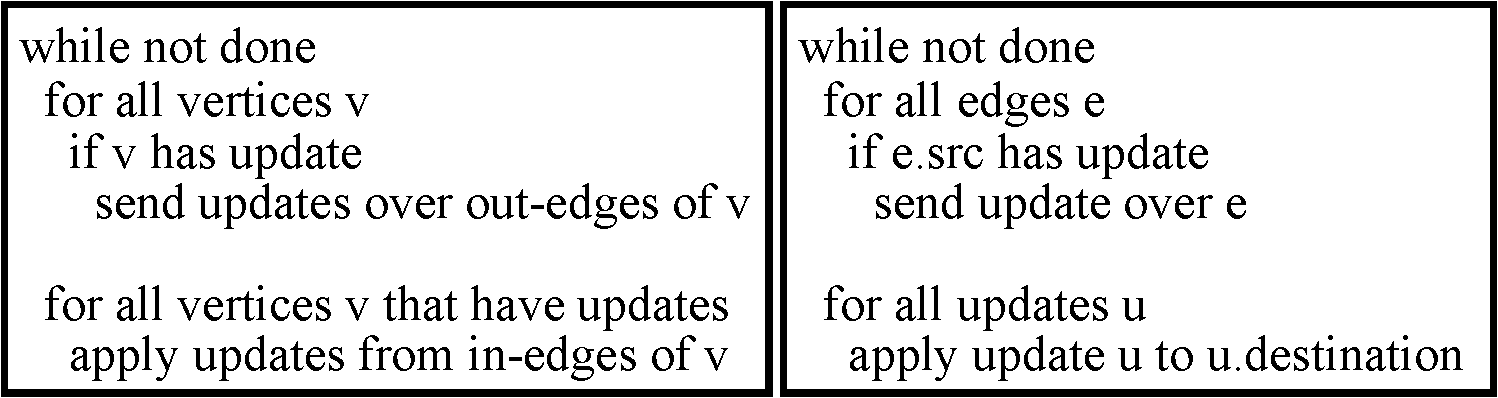
\includegraphics[width=0.75\textwidth]{hybrid-model}
\caption{\small Vertex-centric and Edge-centric Scatter-Gather.}
\label{fig:vertex-edge}
\end{center}
\end{figure}


\subsection{Out-of-Core Graph Processing on GPUs}
\textbf{Hybird Programming Model.}
Figure \ref{fig:vertex-edge} shows two common ways to implement graph algorithms with GAS: edge- vs.vertex-centric execution, which differ in whether the
Scatter and Gather phases iterate over and update edges vs.vertices. GraphLab~\cite{graphlab}, Pregel~\cite{pregel} and GraphChi~\cite{chi} use the vertex-centric model, while X-Stream~\cite{xstream} uses the edge-centric model. In comparison, a more efficient implementation will be to employ a hybrid programming model using both edge- and vertex-centric operations. This is because in the GAS model, different processing phases have different types of parallelism and consequently, offer different parallelism opportunities, coupled with different memory access characteristics. For instance, an edge-centric model should be used in the Gather Phase, because a GPU hardware thread will then be assigned to work on behalf of an edge in the graph. This is preferable to the vertex-centric model, because first, real-world graphs commonly have more edges than vertices, thus giving rise to higher degrees of parallelism and decreased GPU core idling. Second, in the vertex-centric approach, each vertex receives information from multiple in-edges, resulting in a consequent need for synchronization or atomics to order the receive operations from each of the in-edges. This could potentially degrade the overall performance. The same observations hold for using the edge-centric model in the Scatter Phase. In contrast, in the Apply Phase, there are parallelism opportunities only over the vertex set, thus favoring a vertex-centric model.

\label{fig:prob}
\begin{center}
\begin{figure*}[t]
\begin{center}
\begin{minipage}{0.49\textwidth}
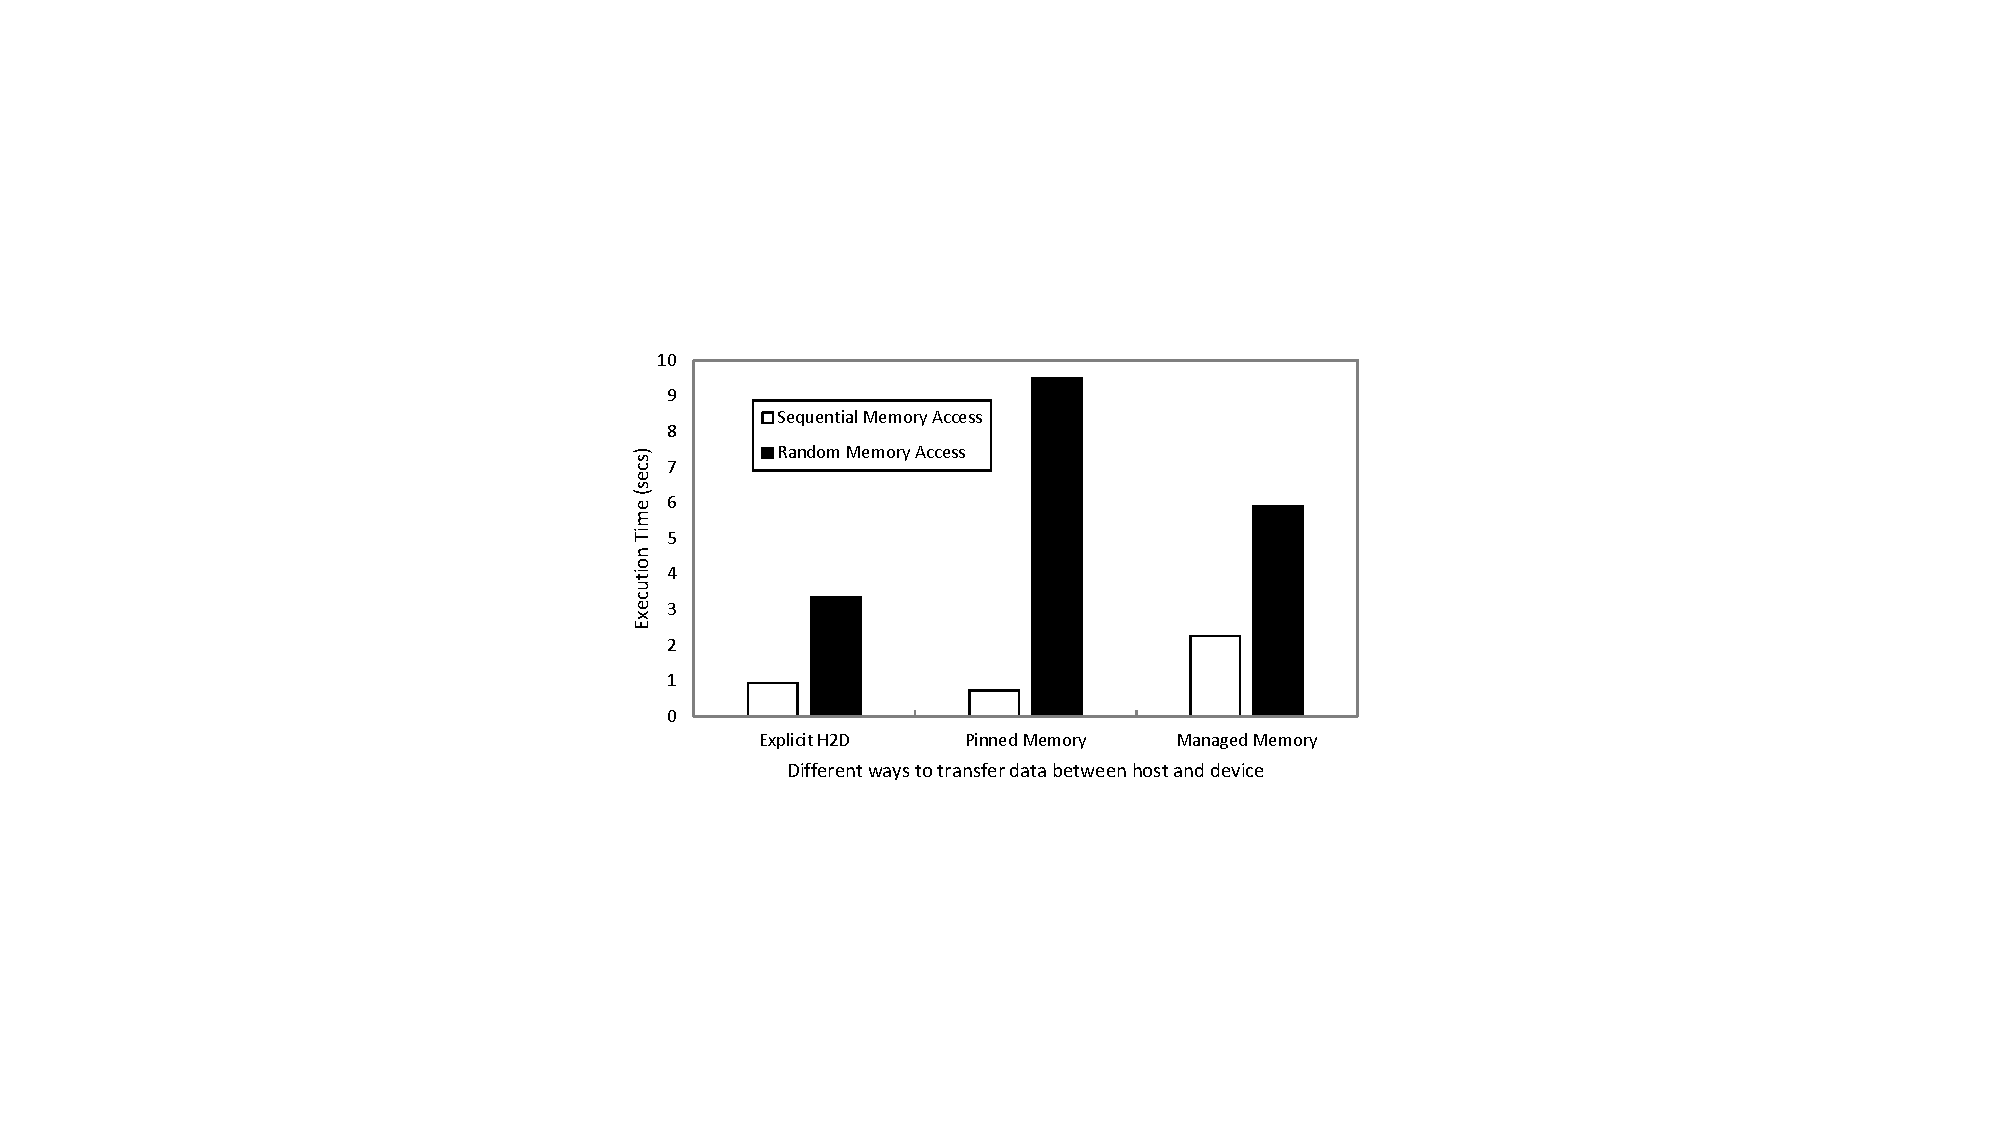
\includegraphics[width=\textwidth, height=4.5cm]{transfer}
\end{minipage}
\begin{minipage}{0.49\textwidth}
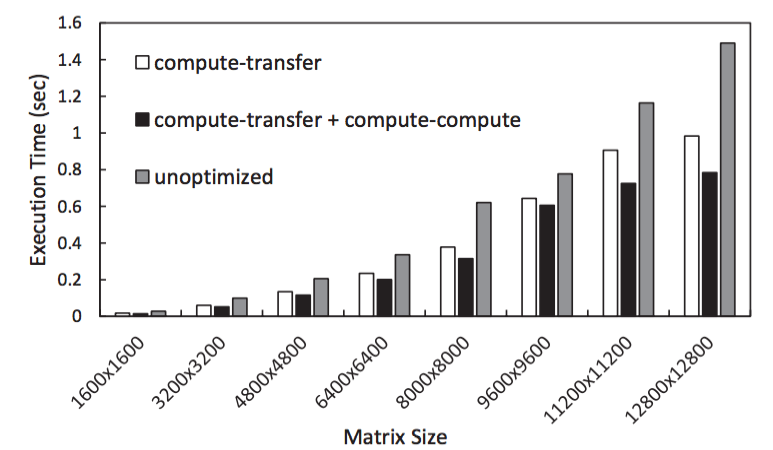
\includegraphics[width=\textwidth, height=5.5cm]{Matrix}
\end{minipage}
\caption{\small a)Performance of transferring 100,000,000 double elements, using three techniques for data exchange between CPU and GPU. b) Performance benefits of using a combination of compute-transfer and compute-compute schemes for processing matrix multiplication with different input sizes. Stripe size=50, which refers to the contiguous number of rows of the matrix being fetched into the GPU memory as a chunk.}
\label{fig:transfer}
\end{center}	
\end{figure*}
\end{center}

\textbf{Characterization of Buffers in Play. }
Graph data chunked to fit into GPU memory and to be moved from host to GPU, is comprised of edges that have either a destination or a source vertex in some well-defined graph partition. Henceforth termed shards, such chunks reside in memory buffers that experience different access patterns. We characterize such access patterns in order to appropriately map corresponding memory buffers to the memory abstractions exposed by current GPUs. In terms of data movement, buffers can be classified as static vs. streaming buffers. Static buffers are copied only once to GPU memory, typically in the Initialization phase. They remain there for the lifetime of the graph execution. An example is a vertex set of a graph that fits into GPU memory. Streaming buffers, on the other hand, are moved in and out of GPU memory as processing progresses, and at any point in time, a particular instance of some streaming buffer resides in GPU memory, e.g., a subset of a graph’s edge set. In the GAS programming model, static buffers are accessed in all three phases, while streaming buffers only appear in a single phase. Another way to characterize buffers is by their access rules, such as read-only or read/write access. For example, vertex and edge data buffers (containing mutable states) have both read and write access patterns, while the vertex set (containing immutable vertex IDs) is read-only. Based on these attributes, the GR runtime makes decisions on whether or not to transfer certain buffers back to the host . Finally, buffers can be classified in terms of the spatial locality of their accesses, e.g., random or sequential access. For example, in the edge-centric approach, there are random accesses to the vertex set.
Once characterized, buffers are mapped to the different memory abstractions exposed by GPU, which at minimum, contain slow and fast memory (e.g., host memory and GPU memory). In the different phases of the GAS model, there are a mix of random and sequential accesses to the input buffers (e.g., edge/vertex sets). For this mix, we posit that random access to slow memory is much more expensive than random access to faster memory, whereas for sequential access, memory-level parallelism and prefetching can help mask slower memory access speed. Therefore, due to the limited fast memory size (GPU), we choose to map all sequential accesses in a GAS phase to the slower CPU memory and all the random accesses to the faster GPU memory. We next validate these assumptions. Figure~\ref{fig:transfer}a. depicts the performance of three techniques for data exchange between host and GPU (through CUDA runtime APIs): (a) explicit data transfer using cudaMemcpy() or Explicit H2D; (b) Pinned Memory using Unified Virtual Addressing (UVA), in which data is transferred implicitly by the CUDA runtime but the memory is allocated as locked memory on the host side; and (c) Managed Memory (introduced in CUDA 6 as Unified memory), where data is transferred between host and device on demand. The measurements shown in the figure illustrate that in the case of sequential memory access, Pinned Memory performs the best, because the accesses directly translate to memory loads/stores operations over the PCIe in which (i) sequential accesses benefit from memory level parallelism (MLP) and (ii) software-level prefetching can hide communication overheads. In the case of random access, Explicit H2D performs the best and Pinned Memory performs the worst. In other words, random access performs best when data resides in faster GPU memory, and the performance of the Pinned Memory degrades as the load/store memory operations over the PCIe fail to benefit from prefetching (after all, accesses are random!). Since Pinned Memory performs the best for sequential accesses, one straightforward approach is to or- ganize graphs such that all memory accesses are sequential. However, because of the significant number of random accesses to either the edges or vertices of a graph in at least one phase of the GAS model, this is not a viable solution for GR as the benefits of sequential accesses are overshadowed by the huge overhead of the random accesses to the slow memory. In response, GR uses explicit data transfer as the mechanism for transferring data between host and device, in way that aim to leverage GPU memory coalescing and software prefetching for the sequential accesses.Although certain performance benefits may exist through intellegent runtime buffer-type selecting. 

\textbf{Coordinated Movement Computation and Data.}
The spatial choice of where in memory to locate data requires an associated temporal choice in when to perform data movement between host and GPU memories. GR uses two methods to attain high performance: (1) hide communication costs by overlapping GPU computation with necessary data transfers, and (2) utilize the GPU’s inherent high degree of potential internal parallelism. (1) is obtained via software-based prefetching to move shards into GPU memory while GPU kernel(s) are being executed. (2) is realized by leveraging underutilized GPU resources (idle threads) caused by the irregular nature of graph processing. It involves (i) detecting such idle threads, using the computation frontier information available to the GR runtime, and (ii) initiating the execution of new shards when idleness is present (note that shards within a single GAS phase do not have data dependencies, so they can be processed in parallel). GR accomplishes this by automatically launching multiple kernels (within the same context), according to the resources available in each GAS phase. Denoting (1) as compute-transfer scheme and (2) as a compute-compute scheme, Figure~\ref{fig:transfer}b. shows the performance benefits obtained from using these approaches vs. an unoptimized scenario when processing a large matrix that doesn’t fit into GPU memory, thus clearly demonstrating the importance of coordinating computation with data movement. We will use these two schemes for processing graph algorithms across phases in the GAS model.

\subsection{Evolving Graph Analytics on GPUs}
There are two major scenarios in terms of analysis of evolving graphs: 1) Offline evolving graph processing where multiple versions of the graph are stored and analyzed to observe the change in certain graph properties over time. 2) Online evolving graph processing that involve real-time continuous query processing over streaming updates on the evolving graph. our solution focuses on online graph analytics. For the rest of the document, evolving graph processing implies online graph analytics.
There are broadly three key characteristics of evolving graphs that dictate the design decisions for our framework:
\begin{itemize}
\item Computation overlap in a sequence of evolving graph versions
\item Data or working set overlap in a sequence of evolving graph versions
\item Static vs dynamic execution runtime
\end{itemize}

{\bf Computation overlap and programming model.}
Between multiple versions or snapshots of an evolving graph the vertex states or values for many vertices remain the same over time and therefore their recomputation is essentially redundant. We define an inconsistent vertex to be a vertex for which one or more properties are affected when the update batch is applied. For example, while calculating out-degree of vertices, an addition or deletion of edge $(v\textsubscript{i},v\textsubscript{j})$ only makes vertex vi inconsistent. For BFS however, addition of edge $(v\textsubscript{i},v\textsubscript{j})$ makes $v\textsubscript{j}$ and all vertices that are “downstream” from $v\textsubscript{j}$ inconsistent. One can consider the entire vertex V to be inconsistent by default. In many scenarios, changes affect only a very small subset of the graph (e.g. calculating out-degree) and computing the vertex states only for those inconsistent vertices and feeding the vertex states from the previous graph versions for the rest of the vertices will significantly reduce the computation time. This observation is the key motivation of the proposing a new programming model for incremental graph processing. To reduce overheads, we aim to build a set of inconsistent vertex sets and sub-graphs that are affected by an update batch and then reduce the incremental graph problem to a sub-problem in the GAS model.

\textbf{Working set overlap and data structure choice.}
When choosing the data structure to store the evolving graph with n vertices and m edges we have multiple options. Adjacency matrices allow for fast update with both insertions and deletions taking O(1) time but require a lot of space O($n\textsuperscript{2}$). Adjacency lists are space efficient O(m+n) and allow fast updates but graph traversals are very inefficient due to non-contiguous memory nodes in the adjacency edge list. Compressed Sparse Row (CSR) formats provide both space efficiency combined with fast traversal (often can be easily parallelized) by storing offsets rather than all the valid fields in the adjacency matrix. But inserts and deletes are very expensive because each update requires shifting of the graph data throughout the compressed array to match the compressed format.
Another key observation to make here is that there is huge overlap in the edge and vertex set between consecutive versions of an evolving graph. Formally, if the graph evolved from G to G’ in certain time epoch t and let $\delta\textsubscript{1} = G' - G$ (insertions), $\delta\textsubscript{2} = G - G'$(deletions) then $G \cap G' = G - \delta\textsubscript{2}   = G' - \delta\textsubscript{1}$ is the overlap between the working set of the two consecutive versions.
In order to allow faster updates to the graph and run both the incremental and static graph algorithms more efficiently, GraphIn uses a hybrid data structure involving edge-lists to store incremental updates and compressed format to store the previous static version of the graph. As mentioned above, the edge-list allows for faster updates, and it does this without adversely affecting the performance of incremental computation. The compressed matrix format allows for faster parallel computation over the entire static version of the graph.  The framework merges the update list and the static graph whenever required.

\textbf{Static vs dynamic runtime.}
Runtime of online graph analytics varies widely depending on the algorithm and the update list. There are scenarios when the incremental algorithm affects only a small or local portion of the graph (e.g., makes a small subset of the graph inconsistent) and changes to the graph require accesses proportional to the size of the update batch. Per-vertex properties that depend on  a fixed radius affect only a local portion of the graph and hence the runtime is proportional to the update batch size (e.g., for triangle counting and in-degree calculation). On the other hand there are classes of incremental algorithms where the graph property depends on paths and can cause a large portion of the graph to become inconsistent, resulting in a complete  recomputation of the graph. In this scenario, incremental processing won’t achieve any performance benefit over  static recomputation and might even result in a performance degradation due to the overheads associated with incremental execution. To handle both the scenarios efficiently,  we need heuristics to select either the incremental or static execution pathway. The decision is made dynamically and taken based on a set of built-in or user-defined graph property checks (e.g., vertex degree information) and the fraction of inconsistent vertices in the update batch that meet the criteria. More precisely, if the update is predicted to require access to and/or affect a small portion of the graph then the incremental execution path is taken, otherwise the update is merged with the static graph and the entire graph is recomputed.  Going back to the BFS example, if 90\% of the inconsistent vertices in an update batch are of high degree, a large portion of the graph is likely to be impacted, so the static execution path is taken. The metadata that is used to decide between static and incremental graph execution is discussed in detail in the architecture section.

